\documentclass[10pt]{beamer}
\usepackage{amsmath,amssymb,longtable,hhline}
\usepackage{mathrsfs}
\usepackage{xcolor}
\usepackage{hyperref}
\usepackage{multicol}
\usepackage{anyfontsize}
\usepackage{minted}

\usemintedstyle{tango}
\newcommand{\ltprgsize}{\fontsize{5}{5}\selectfont}
%\newcommand{\ltprgsize}{\footnotesize}
\setminted{fontsize=\footnotesize{},mathescape}

\definecolor{mygreen}{rgb}{0,0.6,0}
\definecolor{mygray}{rgb}{0.5,0.5,0.5}
\definecolor{mymauve}{rgb}{0.58,0,0.82}

\hypersetup{
    bookmarks=true,         % show bookmarks bar?
    unicode=true,           % non-Latin characters in Acrobat’s bookmarks
    pdftoolbar=false,        % show Acrobat’s toolbar?
    pdfmenubar=false,        % show Acrobat’s menu?
    pdffitwindow=false,     % window fit to page when opened
    pdfstartview={FitH},    % fits the width of the page to the window
    pdftitle={Model Driven Architecture Implementation using Linked Data},    % title
    pdfauthor={Evgeny Cherkashin, Alexey Kopaygorodsky, Ljubica Kazi, Alexey Shigarov, Viacheslav Paramonov},     % author
    pdfsubject={model driven architecture},   % subject of the document
    pdfnewwindow=true,      % links in new PDF window
    colorlinks=true,       % false: boxed links; true: colored links
    linkcolor=red,          % color of internal links (change box color with linkbordercolor)
    citecolor=green,        % color of links to bibliography
    filecolor=magenta,      % color of file links
    urlcolor=blue           % color of external links
}

\usepackage{pifont}

\usetheme{Warsaw}
\usecolortheme{crane}
%\useinnertheme{rectangles}
%\setbeamertemplate{itemize item}{\scriptsize\hbox{\donotcoloroutermaths\ding{113}}}
\definecolor{darkding}{RGB}{200,56,0}
\setbeamertemplate{itemize item}{\scriptsize\hbox{\color{darkding}{\bfseries\ding{113}}}}
\setbeamertemplate{itemize subitem}{\tiny\raise1.5pt\hbox{\donotcoloroutermaths$\blacktriangleright$}}
\setbeamertemplate{itemize subsubitem}{\tiny\raise1.5pt\hbox{\donotcoloroutermaths$\blacktriangleright$}}
\setbeamertemplate{enumerate item}{\insertenumlabel.}
\setbeamertemplate{enumerate subitem}{\insertenumlabel.\insertsubenumlabel}
\setbeamertemplate{enumerate subsubitem}{\insertenumlabel.\insertsubenumlabel.\insertsubsubenumlabel}
\setbeamertemplate{enumerate mini template}{\insertenumlabel}

\beamertemplatenavigationsymbolsempty

\usepackage{iftex,ifxetex}
\ifPDFTeX
  \usepackage[utf8]{inputenc}
  \usepackage[T1]{fontenc}
  \usepackage[russian]{babel}
  \usepackage{lmodern}
  \usefonttheme{serif}
\else
  \ifluatex
    \usepackage{unicode-math}
    \defaultfontfeatures{Ligatures=TeX,Numbers=OldStyle}
    \setmathfont{Latin Modern Math}
    \setsansfont{Linux Biolinum O}
    \setmonofont{Fira Mono}[Scale=MatchLowercase]
    \usefonttheme{professionalfonts}
    % \setmathfont[
    %     Ligatures=TeX,
    %     Scale=MatchLowercase,
    %     math-style=upright,
    %     vargreek-shape=unicode
    %     ]{euler.otf}
  \fi
\fi

%\useoutertheme{split}
%\useinnertheme{rounded}
\setbeamertemplate{background canvas}[vertical shading][bottom=white!80!cyan!20,top=cyan!10]
%\setbeamertemplate{sidebar canvas left}[horizontal shading][left=white!40!black,right=black]

\graphicspath{{pics/}}

\providecommand{\email}[1]{\texttt{#1}}

% --------------------------

\begin{document}

\setbeamertemplate{background canvas}[vertical shading][bottom=white,top=white]
\setbeamercolor{background canvas}{bg=white}

\title[Model Driven Architecture Implementation using Linked Data]{Model Driven Architecture Implementation using Linked Data}
\author[E.~Cherkashin, A.~Kopaygorodsky, L.~Kazi, A.~Shigarov, V.~Paramonov]{\bfseries%
  Evgeny Cherkashin${}^*$, Alexey Kopaygorodsky, Ljubica Kazi, Alexey Shigarov, \underline{Viacheslav Paramonov}}
\institute{\normalsize Institute of System Dynamics and Control Theory, Siberian branch of Russian Academy of Sciences, Irkutsk, Russia\\ University of Novi Sad, Technical faculty <<Mihajlo Pupin>>, Zrenjanin, Serbia\\[1em]
${}^*$\email{\href{mailto:eugeneai@icc.ru}{eugeneai@icc.ru}}%
}
\date[2018]{{}\\
The 24${}^\text{th}$ International Conference on Information\\ and Software Technologies (ICIST 2018)\\
October 4${}^\text{th}$ -- 6${}^\text{th}$, 2018,
Vilnius, Lithuania
}
%\date{\today}
\maketitle
\begin{frame}
  \frametitle{Research objectives}
  \textbf{Main objective} of the research is to construct a MDA technology based on nowadays system modeling visual languages (SysML, BPMN, CMMN) and existing Semantic Web \textbf{vocabularies} and \textbf{technologies}. The following techniques and software are under development:
  \begin{enumerate}
  \item CIM representation with SysML, BPMN, CMMN, and results of source code processing,
  \item CIM, PIM, PSM representation in RDF with existing vocabularies,
  \item transformation implementation with logical language Logtalk,
  \item usage of LOD sources in transformations for obtaining additional semantic data,
  \item generation of documents and user interfaces with LOD markup.
  \end{enumerate}
\end{frame}
\begin{frame}
  \frametitle{Related technologies and standards}
  \begin{itemize}
  \item The most widely used technologies \textbf{ATL} and its predecessor QVT, an OMG standard; developed for XMI to XMI conversion;
  \item Usage of ATL trending to shift to CIM level, \emph{e.g.}, BPMN diagram is converted into set of UML diagrams (PIM); used for construction web-applications, CIM is represented with State and Use case UML-Diagrams.
  \item MDA usage is widening, \emph{e.g.}, for analysis of security aspects of distributed application with logical inference over MDA represented model;
  \item UML is used as CIM/PIM in modeling vocabularies (ontologies); there is an OMG standard specification;
  \item XML specifications are used to describe services, \emph{e.g.} WSDL, WS-BPEL;
  \item MDA is opposed to conceptual programming by Enn Tyugu.
  \end{itemize}

  We describe transformation in Logtalk, representing CIM, PIM and PSM as RDF graphs, allowing non-XMI sources to be used, organizing multi-stage modular transformations.
\end{frame}
\begin{frame}
  \frametitle{Logtalk as transformation definition language}
  We have chosen Logtalk as it
  \begin{itemize}
  \item inherits widely known Prolog language syntax and runtime;
  \item implemented as macro package, performance penalties are about 1.5\%;
  \item has flexible semantics: we can define transformations and constraints within the same syntax;
  \item implement object-oriented knowledge (rules) structuring, encapsulation and replacement;
  \item compositional way of transformation implementation;
  \item powerful engine to post constraints on object-to-object messages (events);
  \item has implementation for many Prolog engines.
  \end{itemize}
  The <<regular>> language allow us to use its libraries not directly related to MDA transformations.
\end{frame}
\begin{frame}[fragile]
  \frametitle{Semantic Web technologies in representation of models
    during transformation}
  \begin{itemize}
  \item Assimilates experience of domain basic researches trending to standardization;
  \item Regular set of triples denote a graph (T-Box, A-Box);
  \item Standard vocabularies are formally described (\verb|rdfs:domain|, \verb|rdfs:range|);
  \item Supported with most programming systems (libraries, inference engines, SPARQL);
  \item RDF has a way of global element identification, \emph{i.e.} we can refer the same object from different software systems;
  \item SWI-Prolog supports direct queries to a graph, as well as interpreting some predicates (\verb|rdfs:label|, \verb|dc:title|), wraps sparse RDF structure into a predicate arguments; ontological server ClioPatria;
  \item There is simple way of data security implementation (\verb|rdfs:seeAlso|);
  \item By means of Semantic Web \& LOD we are able to organize data transfer between heterogeneous information systems.
  \end{itemize}
\end{frame}
\begin{frame}
  \frametitle{Model Driven Architecture and Linked Open Data}
  \begin{center}
    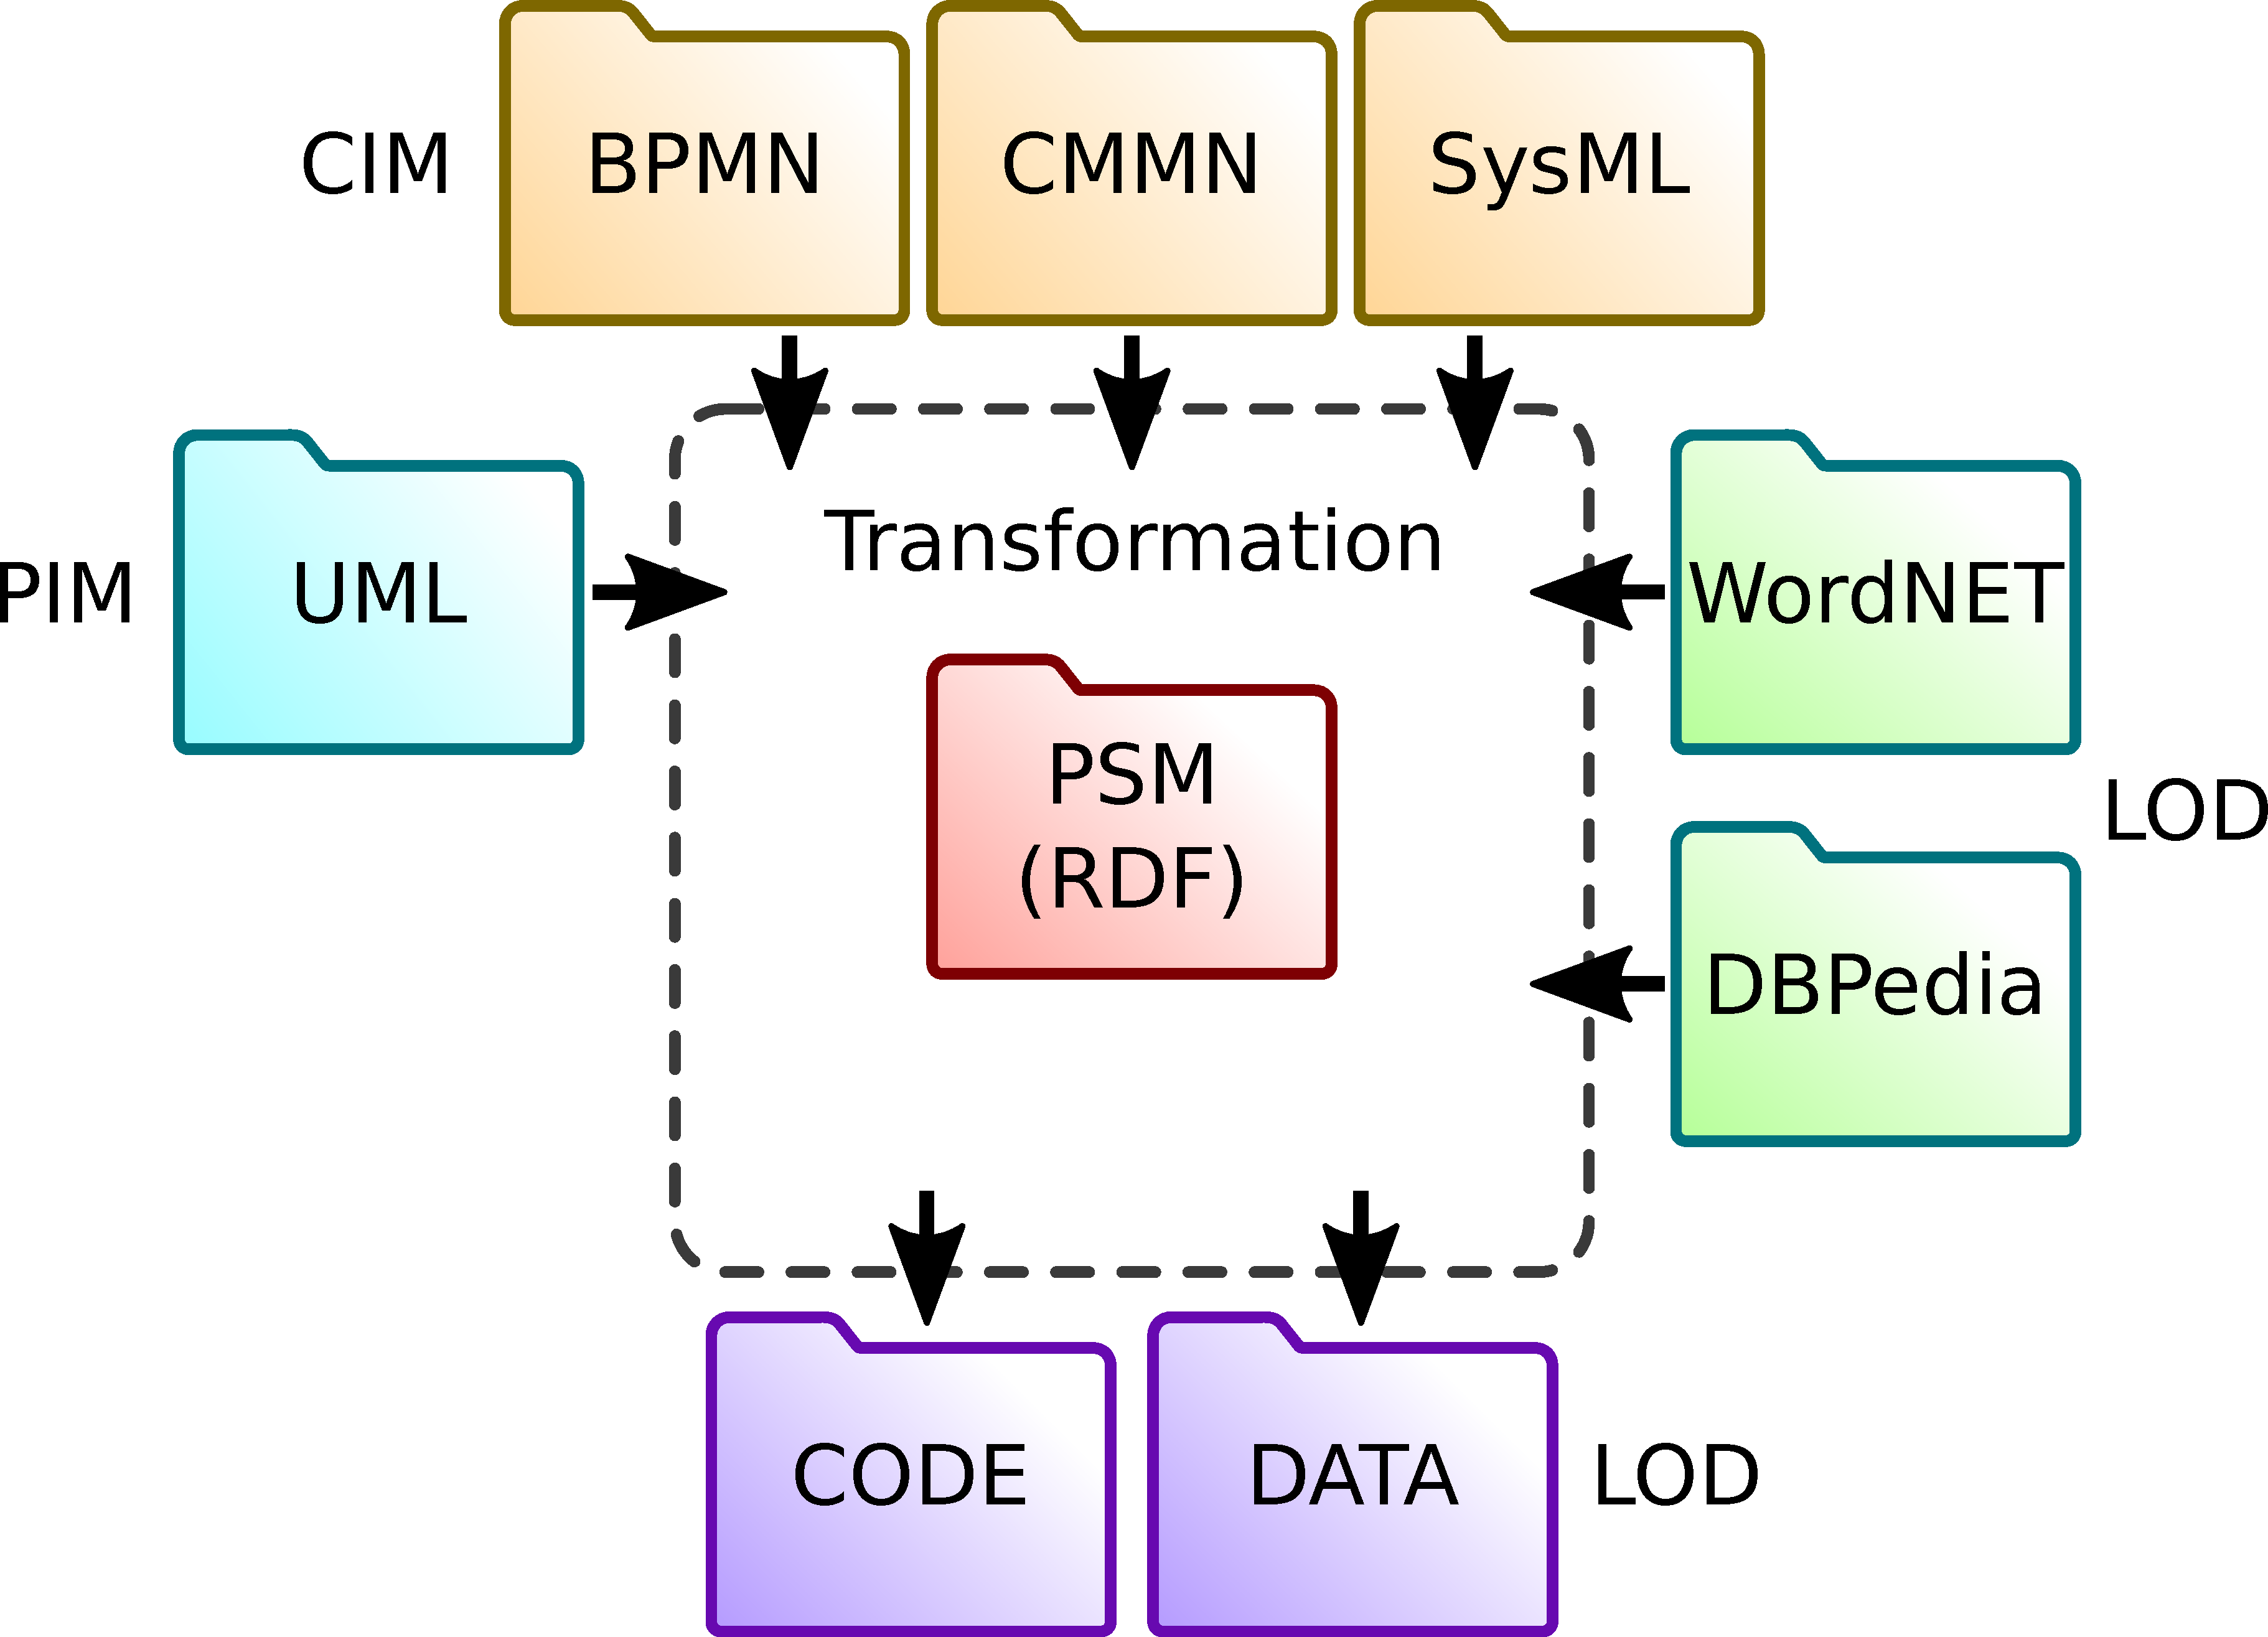
\includegraphics[width=0.9\linewidth]{mda-overview.pdf}
  \end{center}
\end{frame}
\begin{frame}
  \frametitle{MDA infrastructure}
  \centering
  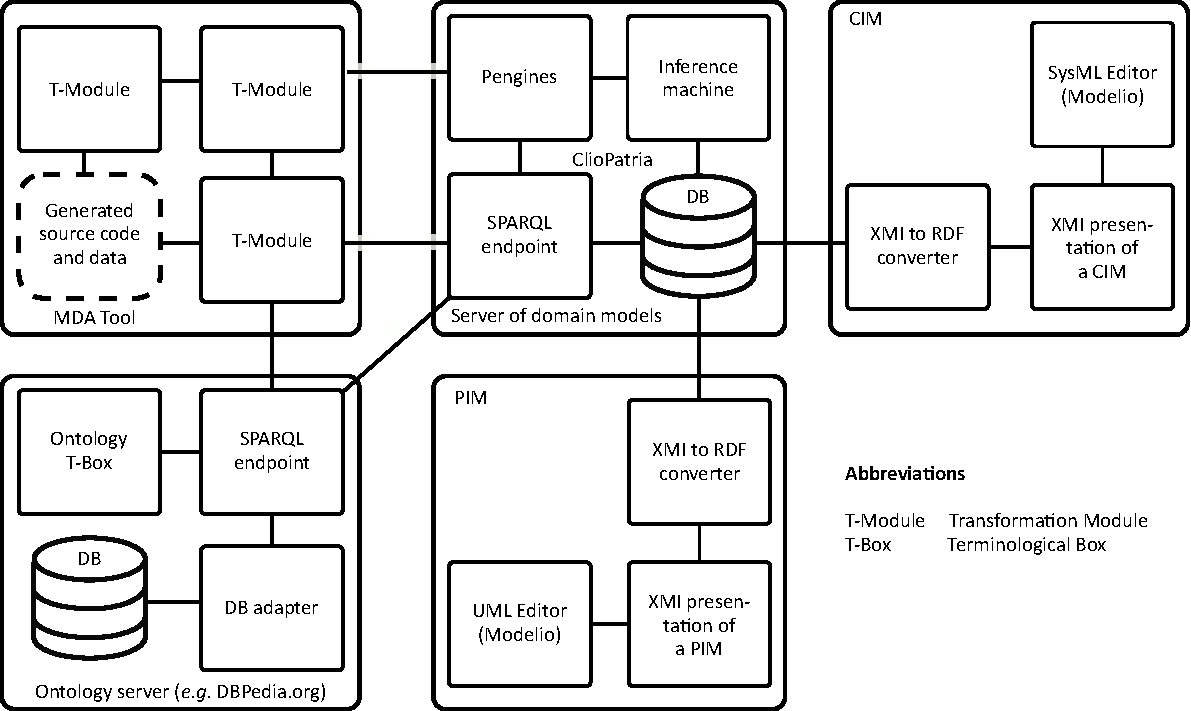
\includegraphics[width=1\linewidth]{architecture-mda-lod-ext.pdf}
\end{frame}
\begin{frame}
  \frametitle{Architecture of transformation modules}
  \centering
  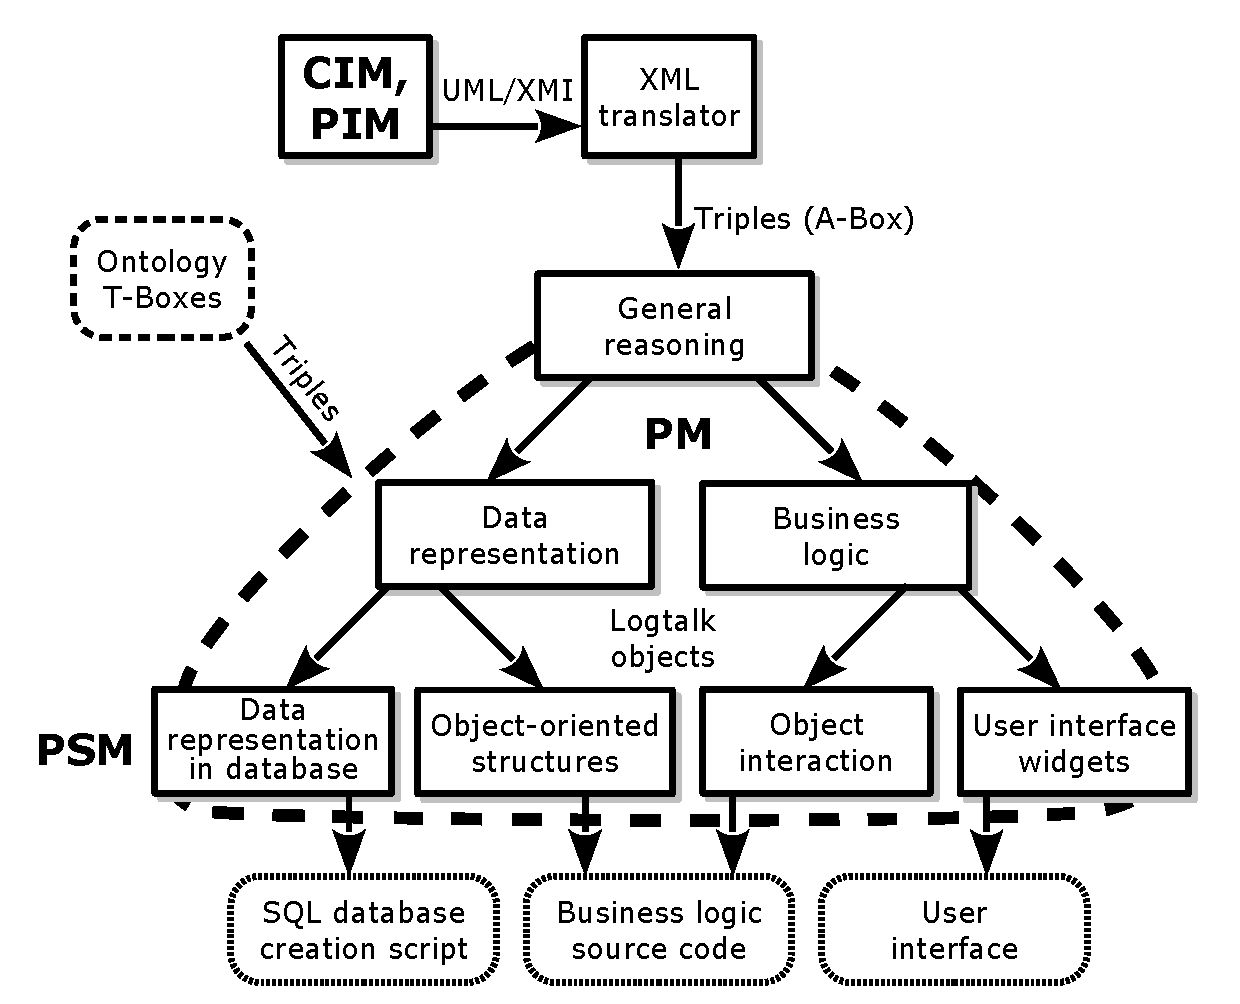
\includegraphics[width=0.9\linewidth]{architect_tree_pres-en-wo-OCL.pdf}
\end{frame}

\begin{frame}[fragile]
  \frametitle{PSM: Scenario of a Class synthesis}

%\begin{multicols}{2}
  \begin{columns}
    \begin{column}{0.6\textwidth}
\begin{minted}[fontsize=\tiny]{logtalk}
:- object(direct(_Package,_LocalProf,_CodeProf)).    % Transformation driver object
:- public([tr/4,tr/3]).                              % Public interface of a class synthesis scenario
% . . . . . . . . . .
tr(class, Class, ClassID):- ::package(Package),      % Synthesize a class
    query(Package)::class(Name, ClassID),            % Query package structure in XMI
    create_object(Class,      % . . . . .            % Create a <<Class>> object
    create_object(Attributes, % . . . . .            % Create <<Attributes>> object
    create_object(Methods,    % . . . . .            % ...<<Methods>>.
    Class::name(Name),                               % Name the class.
    % Generate attributes of the class,
    % organizing them in a local database.
    % ...methods...
    Class::attributes(Attributes),                   % Set the attributes for class.
    Class::methods(Methods).                         % ...methods.

tr(attribute, Attribute, ClassID, AttributeID):-     % Attribute transformations
    ::package(Package),
    query(Package)::attribute(Name,ClassID,AttrID),
    create_object(Attribute,  % . . . . .
    Attribute::name(Name).                           % Name the attribute.

tr(method, Method, ClassID, MethodID):-              % Transformation of methods
    ::package(Package),
    query(Package)::method(Name,ClassID,MethodID),
    create_object(Method,     % . . . . .
    Method::name(Name).                              % Name of the method
:- end_object.
\end{minted}
    \end{column}
    \begin{column}{0.4\linewidth}
      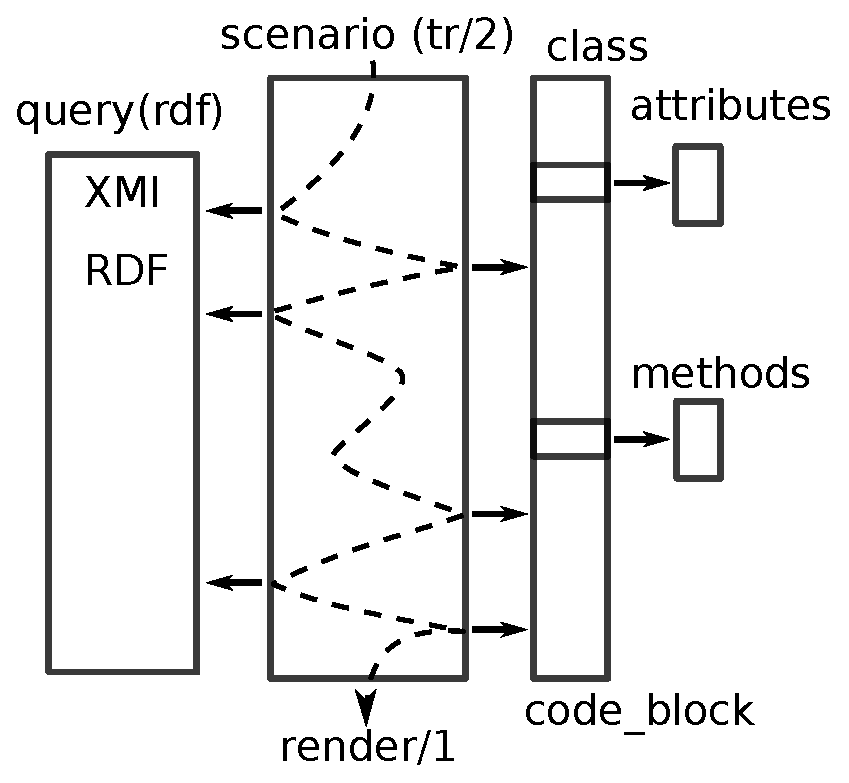
\includegraphics[width=1\linewidth]{scenario.pdf}
    \end{column}
  \end{columns}
  % \end{multicols}
\end{frame}

\begin{frame}[fragile]
  \frametitle{Implementation of \texttt{Query} object}
\begin{minted}[fontsize=\footnotesize{}]{logtalk}
:- object(query(_XMI)).
:- protected(xmi/1).
:- public([class/2, attribute/3, method/3]).
xmi(XMI) :- parameter(1, XMI).
class(Name, ID):-                            % Recognition of Class in RDF
    ::xmi(XMI),
    XMI::rdf(ID,rdf:type,uml:'Class'),
    XMI::rdf(ID,rdfs:label, literal(Name)).
attribute(Name, ClassID, ID):-               % ...attribute...
    ::xmi(XMI),
    XMI::rdf(ClassID, xmi:ownedAttribute, ID),
    XMI::rdf(ID, rdfs:label, literal(Name)).
method(Name, ClassID, ID):-                  % ...method...
    ::xmi(XMI),
    XMI::rdf(ClassID, xmi:ownedOperation, ID),
    XMI::rdf(ID, rdfs:label, literal(Name)).
% . . . . . . . . . . .
:- end_object.
\end{minted}
\end{frame}

\begin{frame}[fragile]
  \frametitle{Code Block (idea is taken from \texttt{llvmlite}${}^*$)}
  \begin{columns}
    \begin{column}{0.6\textwidth}
      \flushleft
\begin{minted}[fontsize=\footnotesize{}]{logtalk}
:- object(code_block, specializes(root)).
% Public interface of the object
:- public([append/1, prepend/1, clear/0,
   render/1, render_to/1, remove/1,
   item/1, items/1]).
% Code block items
:- dynamic([item_/1]).
:- private([item_/1]).
% Methods specialized during inheritance
:- protected([renderitem/2, render_to/2]).
% . . . . . . . . . . . .
% Delegate rendering to object itself
renderitem(Object, String):-
    current_object(Object), !,
    Object::render(String).
% Convert a literal to its string
% representation
renderitem(literal(Item), String):-!,
    atom_string(Item, String).
% Just print the item (debugging).
renderitem(Item, String):-
    root::iswritef(String, '%q', [Item]).
:- end_object.
\end{minted}
    \end{column}
    \begin{column}{0.4\textwidth}
      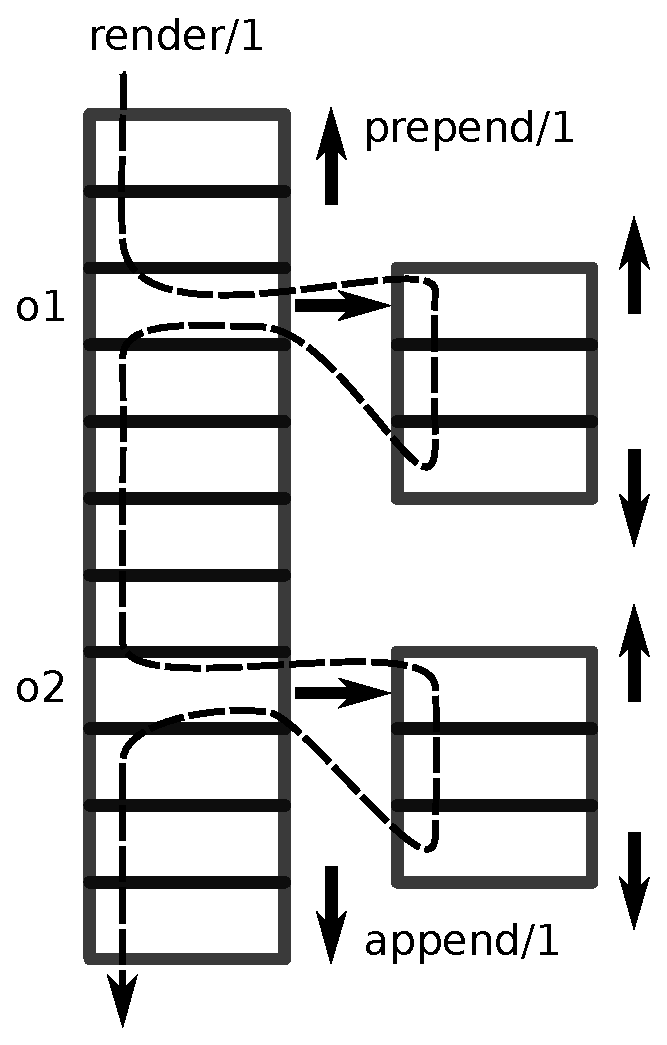
\includegraphics[width=1\linewidth]{code_block.pdf}
  ${}^*$) \url{https://github.com/numba/llvmlite}
    \end{column}
  \end{columns}
\end{frame}

\begin{frame}[fragile]
  \frametitle{PSM of a Python Class as a specialization of Code Block}
%\begin{multicols}{2}
  \begin{columns}
    \begin{column}{0.6\textwidth}
      \flushleft
\begin{minted}[fontsize=\scriptsize]{logtalk}
:- object(class, specializes(code_block),
   imports([named])). % Category of named entities
:- public([classlist/1, methods/1, attributes/1]).
% . . . . . . . . . . . . . .
renderitem(Item, Result):-      % proceed with default
    ^^renderitem(Item, Result). % rendering
render(Result):-         % Source generator
    ^^render(Name),      % implemented in a category
    ( ::item(classlist(List)) ->
     % . . . . . . . . . . .
        [Name]) ),
    ( ::item(attributes(Attributes))->
     % . . . . . . . . . . .
        [DefAttrList]),
      Attributes::items(InstanceAttrs),
      findall(S, ( % initialize attributes
         % . . . . . . . . .
         ), AttrAssigns),
        root::unindent,
        AttrList=[ConstructorDef|AttrAssigns];
         % . . . . . . . . .
        AttrList=[ConstructorDef, Pass] ),
    ( ::item(methods(Methods))-> % If any ...
      Methods::render(MethodList);
      MethodList=[] ),
    lists::append(AttrList,MethodList,StringList),
    root::unindent, Result=[Signature|StringList].
:- end_object.
\end{minted}
    \end{column}
    \begin{column}{0.4\linewidth}
      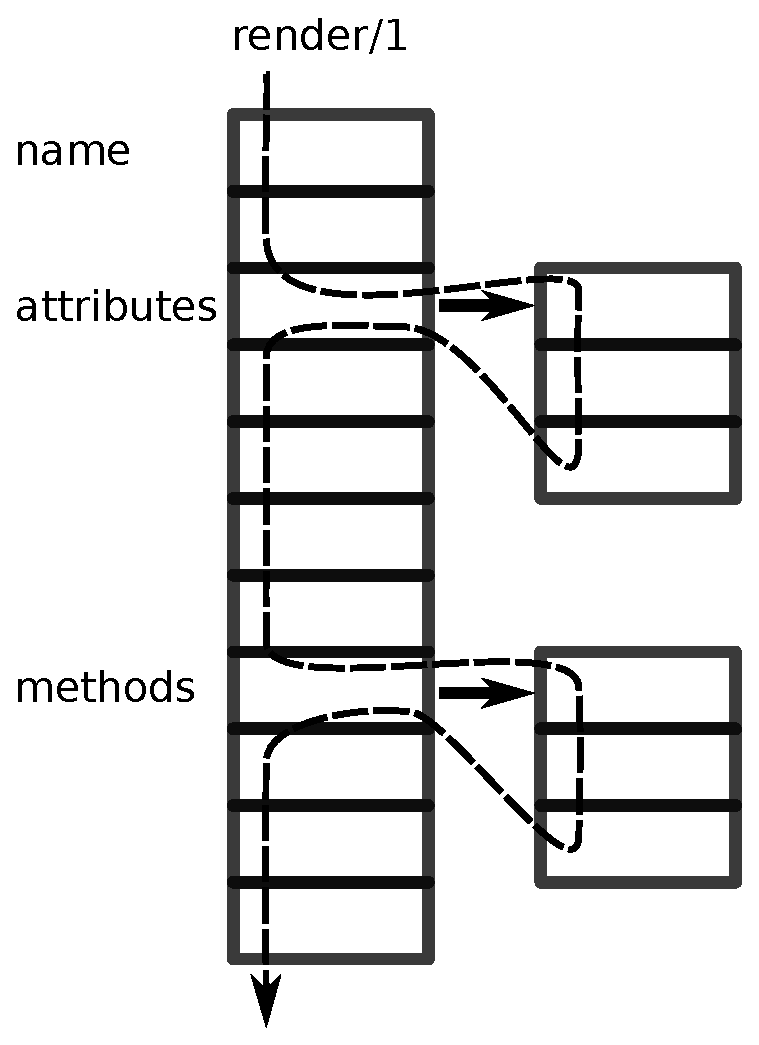
\includegraphics[width=1\linewidth]{code_block_class.pdf}
    \end{column}
  \end{columns}
  % \end{multicols}
\end{frame}

\begin{frame}[fragile]
  \frametitle{Logtalk Categories}
  A category of named entities
\begin{minted}[fontsize=\scriptsize]{logtalk}
:- category(named).
:- public([name/1, render/1]).
:- protected([renderitem/2]).
name(Name):- ::prepend(name(Name)).
renderitem(name(Name), String):-!, atom_string(Name, String).
render(String):-  % What is code generation from items
    ::item(name(Name)), ::renderitem(name(Name), String).
:-end_category.
\end{minted}
Category of named and typed entities
\begin{minted}[fontsize=\scriptsize]{logtalk}
:- category(namedtyped, extends(named)).
:- public([type/1,render/2, separator_option/2,list_separator/1]).
:- protected([renderitem/2]).
type(Type):- ::append(type(Type)).
renderitem(Item, String):- ^^renderitem(Item, String),!.
renderitem(type(Type),String):-!, ::list_separator(Separator),
    writef::swritef(String, '%w%w', [Separator, Type]).
render(Middle, String):- ^^render(SName),
    (   ::item(type(Type)) ->
        ::renderitem(type(Type), SType),
        string_concat(SName, Middle, _1),
        string_concat(_1, SType, String) ;
        SName = String  ).
render(String):-  ::render("", String).
list_separator(Separator):-
    ::separator_option(Name, Default),!, % Global options
    root::option(Name, Separator, Default).
:- end_category.

\end{minted}
\end{frame}

\begin{frame}[fragile]
  \frametitle{Access LOD data}

  \begin{columns}
\begin{column}{0.5\textwidth}
\begin{minted}[fontsize=\scriptsize]{logtalk}
:- category(sparql).
:- public(query/2).
query(Pattern,Parameters,Row):-
    prepare(Pattern,Parameters,Query),
    server(Host,Port,Path),
    sparql_query(Query, Row,
        [host(Host),port(Port),path(Path)]).
:- protected(server/3).  % must be implemented
                         % by a subclass.
:- protected(prepare/3). % prepares a query
% . . . . . . . . . .    %             string.
:- end_category.

:- object(dbpedia, extends(sparql)).
:- protected(server/3).
server('dbpedia.org',80,'/sparql').
:- public(entity_name/2).
entity_name(Entity,Language,Name):-
    query('select ?name where { '
          ' %w rdfs:label ?name. '
          'FILTER langMatches( lang(?label),'
          ' "%w" )}', [Entity, Language],
          row(Name)).
:- end_object.

% ?- dbpedia::entity_name(dbr:'Passport', 'ru', Name).
\end{minted}
\end{column}
\begin{column}{0.5\textwidth}
  \flushright
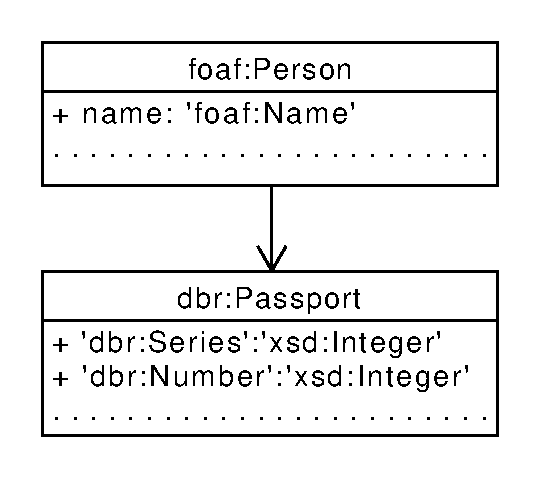
\includegraphics[width=0.8\linewidth]{simple-diag.pdf}
\end{column}
\end{columns}
\end{frame}


\begin{frame}
  \frametitle{Applications: Dataflow representation of NGS analysis of amplicons}
  \begin{columns}
    \begin{column}{0.6\textwidth}
      \begin{raggedright}
        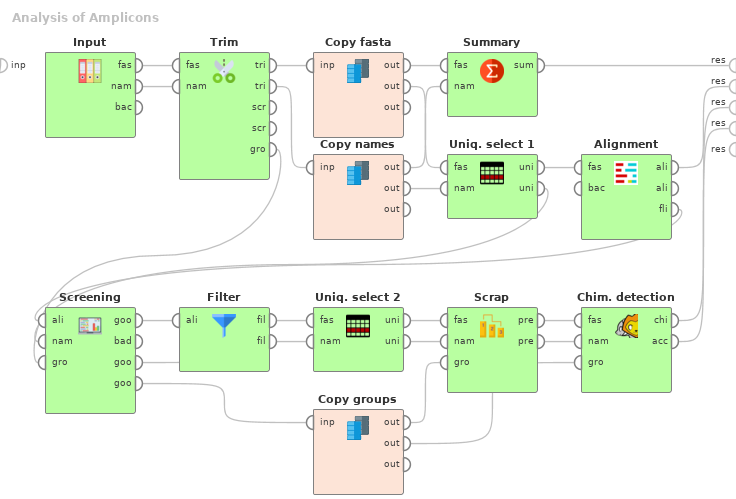
\includegraphics[width=1\linewidth]{Dataflow-color-en.png}
      \end{raggedright}
    \end{column}
    \begin{column}{0.4\textwidth}\footnotesize
      \begin{tabular}{ll}
        Term & Description \\
        \hline
        NGS & New Generation\\ & Sequencing\\
        Amplicon & A DNA or RNA part \\
                 & copied many times \\
        Mothur & A software toolset for\\ & NGS research \\
        Rapidminer & A visual tool for \\
             & data mining modeling\\
             &  and execution
      \end{tabular}
      ${}$\\[1em]
      Green blocks are Mothur modules. Others are Rapidminer modules.
    \end{column}
  \end{columns}
\end{frame}


\begin{frame}
  \frametitle{Discussion}
  Interesting positive impressions obtained:
  \begin{itemize}
  \item Logtalk and RDF are flexible, sufficiently universal and convenient implementation infrastructures for MDA;
  \item The best implemenation means is Prolog predicate wrapping and Logtalk object encapsulation of rules;
  \item Not all Logtalk properties are investigated: there might be more sophisticated programming techniques developed, \emph{e.g.}, on the base of message watchers.
  \end{itemize}
  Technical problems making the approach somewhat problematic:
  \begin{itemize}
  \item Very simple tasks take too much efforts, \emph{e.g.}, text processing: convert an identifier into the CamelCase;
  \item It takes too long to surf Internet in order to find a vocabulary for a domain, but it is more productive than development;
  \item Prolog is not a popular language in MDA, neither Logtalk.
  \end{itemize}
\end{frame}

\begin{frame}
  \frametitle{Conclusion}
  The following results have been obtained as for today:
  \begin{itemize}
  \item A technique for model representation has been developed and tested.
  \item A programming technique using object-oriented logical language Logtalk is deviced.
  \item Ptototypes of various transformation procedures are implemented.
  \item Transformation tools are tested in application areas and no significant technical problems were mentioned.
  \end{itemize}
  Further development directions are as follows:
  \begin{itemize}
  \item A technique for document automatic markup with vocabulary entities.
  \item A transformation implemenation techniques, minimizing usage of dynamic objects, targeting on macro properties of Logtalk.
  \item Form a toolset out of existing prototypes obeing nowadays software development requirements.
  \end{itemize}
  The source codes are available at \url{https://github.com/isu-enterprise/icc.xmitransform}, \url{https://github.com/eugeneai/icc.mothurpim}.
\end{frame}

\begin{frame}
  \begin{center}
  \Large Thanks for Your interest to our project!
\end{center}
\end{frame}

\begin{frame}[fragile]
  \frametitle{Rapidminer module}
\begin{minted}[fontsize=\tiny]{cpp}
vector<string> AlignCommand::setParameters(){ // PART OF MODULE SOURCE
try {
  CommandParameter ptemplate("reference", "InputTypes", "", "", "none", "none", "none","",false,true,true); parameters.push_back(ptemplate);
  CommandParameter pcandidate("fasta", "InputTypes", "", "", "none", "none", "none","fasta-alignreport-accnos",false,true,true); parameters.push_back(pcandidate);
  CommandParameter psearch("search", "Multiple", "kmer-blast-suffix", "kmer", "", "", "","",false,false,true); parameters.push_back(psearch);
  CommandParameter pksize("ksize", "Number", "", "8", "", "", "","",false,false); parameters.push_back(pksize);
  CommandParameter pmatch("match", "Number", "", "1.0", "", "", "","",false,false); parameters.push_back(pmatch);
// . . . . . . .
\end{minted}
\begin{minted}[fontsize=\tiny]{java}
package com.rapidminer.ngs.operator; // GENERATED JAVA MODULE
// imports

class MothurChimeraCcodeOperator extends MothurGeneratedOperator {
  private InputPort fastaInPort = getInputPorts().createPort("fasta");
  private InputPort referenceInPort = getInputPorts().createPort("reference");
  private OutputPort chimeraOutPort = getOutputPorts().createPort("chimera");
  private OutputPort mapinfoOutPort = getOutputPorts().createPort("mapinfo");
  private OutputPort accnosOutPort = getOutputPorts().createPort("accnos");

  public MothurChimeraCcodeOperator (OperatorDescription description) {
    super(description);
  }
  @Override
  public void doWork() throws OperatorException {
    super();
    // . . . . . .
  }
  @Override
  public List<ParameterType> getParameterTypes() {
    super();
        // . . . . . .
  }
  @Override
  public String getOutputPattern(String type) {
    if (type=="chimera") return "[filename],[tag],ccode.chimeras-[filename],ccode.chimeras";
    if (type=="mapinfo") return "[filename],mapinfo";
    if (type=="accnos") return "[filename],[tag],ccode.accnos-[filename],ccode.accnos";
    return super.getOutputPattern(type);
  }
}
\end{minted}
\end{frame}

\begin{frame}[fragile]
  \frametitle{RDF (TTL) representation and ad its query object}
\begin{multicols}{2}
\begin{minted}[fontsize=\tiny]{turtle}
@prefix xml: <http://www.w3.org/XML/1998/namespace> .
@prefix xsd: <http://www.w3.org/2001/XMLSchema#> .
ngsp:spec a ngsp:Specification ;
    ngsp:module mothur:NoCommand,
        mothur:align-check,
        mothur:align-seqs,
# . . . . .
mothur:align-check a ngsp:Module ;
    ngsp:outputPattern [ a cnt:Chars ;
            ngsp:parameterName "type" ;
            ngsp:pattern [ ngsp:patternString
                    "[filename],align.check" ;
                    dc:identifier "aligncheck" ] ;
            cnt:chars # . . . .
# . . . . .
mothur:align-check-idir-parameter a ngsp:Parameter ;
    ngsp:important false ;
    ngsp:multipleSelectionAllowed false ;
    ngsp:optionsDefault "" ;
    ngsp:required false ;
    ngsp:type mothur:String ;
    dc:title "inputdir" .

mothur:align-check-map-parameter a ngsp:Parameter ;
    ngsp:important true ;
    ngsp:multipleSelectionAllowed false ;
    ngsp:optionsDefault "" ;
    ngsp:required true ;
    ngsp:type mothur:InputTypes ;
    dc:title "map" .

mothur:align-check-name-parameter a ngsp:Parameter ;
    ngsp:chooseOnlyOneGroup "namecount" ;
    ngsp:important false ;
    ngsp:multipleSelectionAllowed false ;
# . . . . .
\end{minted}
\begin{minted}[fontsize=\tiny]{logtalk}
:- object(queryparam(_RDF,_Parameter),
          extends(ngsquerybase)).

:- public(type/1).
type(Type) :-
    ::attr(type, Type).
:- public(name/1).
name(Name) :- ::attr(dc:title, literal(Name)).
:- public(options/1).
options(Value):- ::attr(options, Value).
:- public(options_default/1).
options_default(Value):-
    ::attr(optionsDefault, Value).
% . . . . . . . .
:- public(multiple_selection_allowed/0).
multiple_selection_allowed:-
    ::bool_attr(multipleSelectionAllowed).
:- public(required/0).
required:-
    ::bool_attr(required).
:- public(important/0).
important:-
    ::bool_attr(important).
:- protected(attr/2).
attr(NS:Name, Value):-
    ::ngs(RDF),
    ::second(Parameter),
    rdf_db::rdf_global_object(Value, V),
    RDF::rdf(Parameter, NS:Name, V).
attr(Name, Value):-
    \+ Name=_:_,!,
    ::ngs(RDF),
    ::second(Parameter),
    rdf_db::rdf_global_id(Value, V),
    RDF::rdf(Parameter, ngsp:Name, V).
% . . . . .
:- end_object.

\end{minted}
\end{multicols}
\end{frame}


\end{document}

%%% Local Variables:
%%% mode: latex
%%% TeX-master: t
%%% End:
